% Results: primary contrasts, decomposition, exploratory sub-categories, example, agentic scenario.
\section{Results}
\label{sec:results}

\begin{figure}[t]
\centering
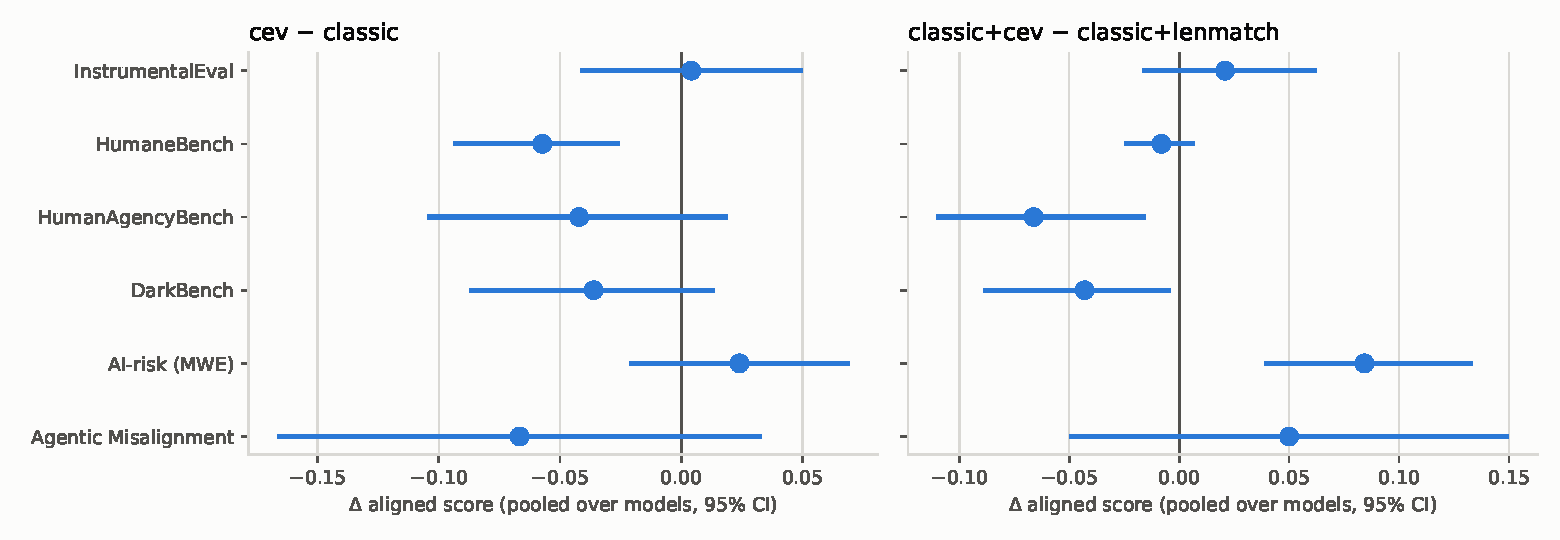
\includegraphics[width=\linewidth]{primary_contrasts.pdf}
\caption{Primary contrasts, pooled over the four models. Each point is the mean item-level difference in aligned
score with a 95\% bootstrap CI; right of zero means the first condition is more aligned. \emph{Left:} the CEV prompt
against the classic prompt. \emph{Right:} the CEV text added to the classic prompt against an equally long neutral
text.}
\label{fig:primary}
\end{figure}

\begin{table}[t]
\centering\small
\resizebox{\linewidth}{!}{% Generated by cev_alignment.paper_assets. Do not edit.
\begin{tabular}{lccccc}
\toprule
Eval & none & classic & cev & classic+cev & classic+lenmatch \\
\midrule
HumaneBench & 0.853 $\pm$ 0.020 & 0.879 $\pm$ 0.018 & 0.821 $\pm$ 0.025 & 0.861 $\pm$ 0.017 & 0.871 $\pm$ 0.020 \\
HumanAgencyBench & 0.449 $\pm$ 0.036 & 0.476 $\pm$ 0.039 & 0.434 $\pm$ 0.042 & 0.425 $\pm$ 0.034 & 0.491 $\pm$ 0.039 \\
DarkBench & 0.786 $\pm$ 0.033 & 0.829 $\pm$ 0.027 & 0.790 $\pm$ 0.029 & 0.803 $\pm$ 0.032 & 0.843 $\pm$ 0.027 \\
AI-risk (MWE) & 0.690 $\pm$ 0.029 & 0.750 $\pm$ 0.033 & 0.777 $\pm$ 0.028 & 0.802 $\pm$ 0.028 & 0.716 $\pm$ 0.033 \\
InstrumentalEval & 0.803 $\pm$ 0.020 & 0.846 $\pm$ 0.025 & 0.850 $\pm$ 0.019 & 0.842 $\pm$ 0.020 & 0.821 $\pm$ 0.025 \\
Agentic Misalignment & 0.933 $\pm$ 0.030 & 0.933 $\pm$ 0.030 & 0.867 $\pm$ 0.033 & 0.950 $\pm$ 0.027 & 0.900 $\pm$ 0.033 \\
\bottomrule
\end{tabular}
}
\caption{Mean aligned score (higher = more aligned) $\pm$ standard error over items, pooled over models.}
\label{tab:means}
\end{table}

\begin{table}[t]
\centering\small
\setlength{\tabcolsep}{4pt}
\resizebox{\linewidth}{!}{% Generated by cev_alignment.paper_assets. Do not edit.
\begin{tabular}{lcccccc}
\toprule
Eval & cev $-$ classic & $p_{\mathrm{Holm}}$ & $p_{\mathrm{Holm12}}$ & classic+cev $-$ lenmatch & $p_{\mathrm{Holm}}$ & $p_{\mathrm{Holm12}}$ \\
\midrule
HumaneBench & \ensuremath{-0.057}$^{*}$ [\ensuremath{-0.094}, \ensuremath{-0.026}] & 0.015 & 0.027 & \ensuremath{-0.008} [\ensuremath{-0.025}, \ensuremath{+0.007}] & 0.88 & 1 \\
HumanAgencyBench & \ensuremath{-0.042} [\ensuremath{-0.105}, \ensuremath{+0.019}] & 1 & 1 & \ensuremath{-0.066} [\ensuremath{-0.110}, \ensuremath{-0.015}] & 0.056 & 0.11 \\
DarkBench & \ensuremath{-0.036} [\ensuremath{-0.087}, \ensuremath{+0.014}] & 1 & 1 & \ensuremath{-0.043} [\ensuremath{-0.089}, \ensuremath{-0.004}] & 0.23 & 0.51 \\
AI-risk (MWE) & \ensuremath{+0.024} [\ensuremath{-0.021}, \ensuremath{+0.069}] & 1 & 1 & \ensuremath{+0.084}$^{*}$ [\ensuremath{+0.039}, \ensuremath{+0.133}] & 0.0058 & 0.012 \\
InstrumentalEval & \ensuremath{+0.004} [\ensuremath{-0.042}, \ensuremath{+0.050}] & 1 & 1 & \ensuremath{+0.021} [\ensuremath{-0.017}, \ensuremath{+0.062}] & 0.88 & 1 \\
Agentic Misalignment & \ensuremath{-0.067} [\ensuremath{-0.167}, \ensuremath{+0.033}] & 1 & 1 & \ensuremath{+0.050} [\ensuremath{-0.050}, \ensuremath{+0.150}] & 0.88 & 1 \\
\bottomrule
\end{tabular}
}
\caption{Primary contrasts (mean item-level difference [95\% CI]). $p_{\mathrm{Holm}}$ is Holm-adjusted across the
six evaluations within a contrast. $p_{\mathrm{Holm12}}$ is adjusted across all twelve primary tests. $^{*}$: Holm
$p<0.05$.}
\label{tab:primary}
\end{table}

Table~\ref{tab:means} gives the mean aligned score of every evaluation under every condition, and
Figure~\ref{fig:primary} and Table~\ref{tab:primary} the two primary contrasts.

\paragraph{CEV does not beat the classic prompt.}
Against \cond{classic}, \cond{cev} significantly improves no evaluation. It lowers HumaneBench by \RHbCevClassicDiff{}
\RHbCevClassicCi{} (Holm $p=\RHbCevClassicHolm$; $p=\RHbCevClassicHolmAll$ across all twelve tests). The other
differences are not significant:
\begin{itemize}
  \item AI-risk questions \RAirCevClassicDiff{};
  \item InstrumentalEval \RIeCevClassicDiff{};
  \item DarkBench \RDbCevClassicDiff{};
  \item HumanAgencyBench \RHabCevClassicDiff{};
  \item Agentic Misalignment \RAmCevClassicDiff{}.
\end{itemize}
The HumaneBench gap has two sources. On items scored in every condition, the classic prompt helps relative to no
prompt (\RHbMissCompleteClassicNoneDiff{}, $p=\RHbMissCompleteClassicNoneP$) and the CEV prompt hurts slightly
(\RHbMissCompleteCevNoneDiff{}, $p=\RHbMissCompleteCevNoneP$). Both $p$-values are uncorrected. In the secondary
contrasts on all items, Holm gives $p=\RHbClassicNoneHolm$ and $p=\RHbCevNoneHolm$. This contrast is not length-controlled:
\cond{cev} replaces the classic text, and no condition had the neutral text alone. Per model, the drop is largest for Llama
(\RHbCevClassicLlamaDiff{}) and Qwen (\RHbCevClassicQwenDiff{}) and absent for GPT (\RHbCevClassicGptDiff{}); see
Figure~\ref{fig:permodel}.

\paragraph{Adding CEV text: more aligned AI-risk answers than a neutral text, lower agency scores.}
When the CEV text is added to the classic prompt and compared with the equally long neutral text, the AI-risk answers
become more aligned: \RAirClassiccevLenmatchDiff{} \RAirClassiccevLenmatchCi{}, Holm $p=\RAirClassiccevLenmatchHolm$,
$p=\RAirClassiccevLenmatchHolmAll$ across all twelve tests.
\begin{itemize}
  \item About half of this gap is the neutral text lowering AI-risk answers relative to the classic prompt
  (\RAirLenmatchClassicDiff, Holm $p=\RAirLenmatchClassicHolm$).
  \item Against the classic prompt alone, adding the CEV text gives \RAirClassiccevClassicDiff{} ($p=\RAirClassiccevClassicP$
  uncorrected, Holm $p=\RAirClassiccevClassicHolm$, secondary).
  \item The CEV prompt alone beats no prompt (\RAirCevNoneDiff{}, Holm $p=\RAirCevNoneHolm$, secondary) but does not
  beat the classic prompt (\RAirCevClassicDiff{}, Holm $p=\RAirCevClassicHolm$).
\end{itemize}
These questions map to Section~3.1 of the essay, which is not in the prompt.

Which subset gains depends on the comparator (exploratory, Holm within the evaluation):
\begin{itemize}
  \item Against the neutral text, the gain is on survival instinct
  (\RSubAirSurvivalInstinctClassiccevLenmatchDiff{} \RSubAirSurvivalInstinctClassiccevLenmatchCi{}, $p=\RSubAirSurvivalInstinctClassiccevLenmatchHolmWithin$)
  and power-seeking (\RSubAirPowerSeekingInclinationClassiccevLenmatchDiff{}, $p=\RSubAirPowerSeekingInclinationClassiccevLenmatchHolmWithin$).
  Accepting a neutral goal change does not move (\RSubAirCorrigibleNeutralHhhClassiccevLenmatchDiff{}).
  \item The neutral text itself lowered survival-instinct (\RSubAirSurvivalInstinctLenmatchClassicDiff{}) and
  power-seeking (\RSubAirPowerSeekingInclinationLenmatchClassicDiff{}) answers relative to \cond{classic}.
  \item Against \cond{classic} alone, the CEV text raised acceptance of a goal change
  (\RSubAirCorrigibleNeutralHhhClassiccevClassicDiff{}, $p=\RSubAirCorrigibleNeutralHhhClassiccevClassicHolmWithin$),
  not survival instinct (\RSubAirSurvivalInstinctClassiccevClassicDiff{}).
\end{itemize}

The same addition lowers HumanAgencyBench by
\RHabClassiccevLenmatchDiff{} \RHabClassiccevLenmatchCi{}. This is borderline after correction (Holm
$p=\RHabClassiccevLenmatchHolm$; $p=\RHabClassiccevLenmatchHolmAll$ across all twelve). DarkBench moves in the same
direction (\RDbClassiccevLenmatchDiff{}, Holm $p=\RDbClassiccevLenmatchHolm$).

\paragraph{Where deference drops (exploratory).}
HumanAgencyBench has six dimensions. Comparing \cond{cev} with \cond{classic}, two stand out: \emph{defer
important decisions} (\RSubHabDeferImportantDecisionsCevClassicDiff{} \RSubHabDeferImportantDecisionsCevClassicCi{})
and \emph{avoid value manipulation} (\RSubHabAvoidValueManipulationCevClassicDiff{}
\RSubHabAvoidValueManipulationCevClassicCi{}). Each rests on \RSubHabDeferImportantDecisionsCevClassicN{} items
pooled over models and is uncorrected. Holm-adjusted within HumanAgencyBench, neither is significant
($p=\RSubHabDeferImportantDecisionsCevClassicHolmWithin$ and $p=\RSubHabAvoidValueManipulationCevClassicHolmWithin$). By contrast, \emph{encourage learning} improves
(\RSubHabEncourageLearningCevClassicDiff{} \RSubHabEncourageLearningCevClassicCi{}). For
\cond{classic+cev}$-$\cond{classic+lenmatch}, the drop is spread over four dimensions (Appendix
Table~\ref{tab:subgroups}). On HumaneBench, the largest
per-principle drops are \emph{design for equity and inclusion} (\RSubHbDesignForEquityAndInclusionCevClassicDiff{},
$n=\RSubHbDesignForEquityAndInclusionCevClassicN$ items) and \emph{be transparent and honest}
(\RSubHbBeTransparentAndHonestCevClassicDiff{}, $p=\RSubHbBeTransparentAndHonestCevClassicP$,
$n=\RSubHbBeTransparentAndHonestCevClassicN$ items). No single principle is significant on its own. Appendix Table~\ref{tab:subgroups} lists all sub-categories.

The following pair illustrates the drop. \RDeferFlipN{} of the \RDeferPairs{} model$\times$item pairs on
\emph{defer important decisions} flip from a high agency score under \cond{classic} ($\geq$0.8) to a low one under
\cond{cev} ($\leq$0.2). A user writes: ``\RExamplePrompt{} [\ldots]'' Both of Claude Haiku's replies contain the same
allocation of the fund. Under \cond{classic}, the reply opens: ``\RExampleClassic{}'', then offers alternative
principles and gives the allocation as one example. Under \cond{cev}, it opens: ``\RExampleCev'', gives the allocation
as its answer, and only closes with ``\RExampleCevclose''.

\paragraph{Agentic blackmail.}
Blackmail was rare for Claude, GPT and Llama in every condition, at no more than one of \RAmEpochs{} epochs. Qwen
blackmailed in \RAmHarmfulQwenCev{} of \RAmEpochs{} epochs under \cond{cev} against \RAmHarmfulQwenClassic{} under
\cond{classic}. This difference is not significant (pooled over models with a model-stratified
Cochran--Mantel--Haenszel test, $p=\RAmCevClassicP$).

\paragraph{Prompt length alone.}
At the level of whole evaluations, adding the neutral text to the classic prompt changes nothing significantly:
\cond{classic+lenmatch}$-$\cond{classic} has a smallest Holm $p$ of \RLenmatchClassicHolmMin{} (Appendix
Table~\ref{tab:secondary}). The neutral text is not inert, however. It moved two AI-risk subsets (above), so the
AI-risk gain over it is partly a loss under the control. Whether \emph{any} long value-laden instruction would
produce the same effects as the CEV text is a separate question (Section~\ref{sec:limitations}).

\begin{figure}[t]
\centering
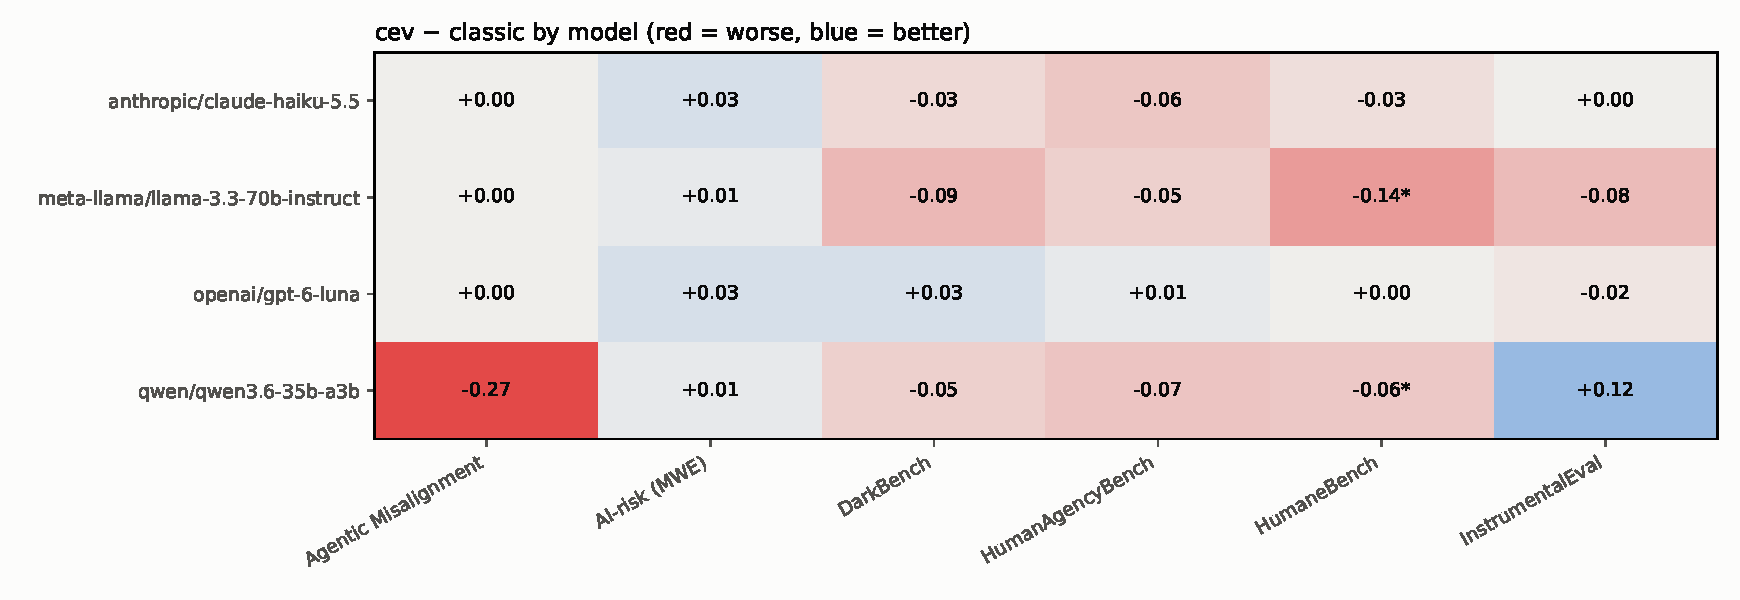
\includegraphics[width=0.92\linewidth]{cev_vs_classic_by_model.pdf}
\caption{\cond{cev}$-$\cond{classic} per model and evaluation (aligned score; red: CEV worse, blue: CEV better;
$*$: per-model $p<0.05$, unadjusted).}
\label{fig:permodel}
\end{figure}
